% This file was created with tikzplotlib v0.10.1.
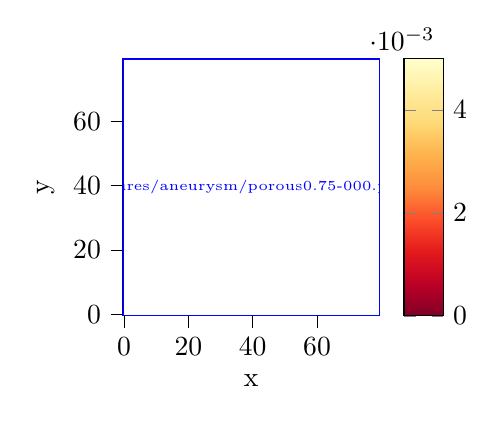
\begin{tikzpicture}
\pgfplotsset{%
    width=0.4\textwidth,
    height=0.4\textwidth
}
\definecolor{darkgray176}{RGB}{176,176,176}

\begin{axis}[
colorbar,
colorbar style={ylabel={}},
colormap={mymap}{[1pt]
  rgb(0pt)=(0.501960784313725,0,0.149019607843137);
  rgb(1pt)=(0.741176470588235,0,0.149019607843137);
  rgb(2pt)=(0.890196078431372,0.101960784313725,0.109803921568627);
  rgb(3pt)=(0.988235294117647,0.305882352941176,0.164705882352941);
  rgb(4pt)=(0.992156862745098,0.552941176470588,0.235294117647059);
  rgb(5pt)=(0.996078431372549,0.698039215686274,0.298039215686275);
  rgb(6pt)=(0.996078431372549,0.850980392156863,0.462745098039216);
  rgb(7pt)=(1,0.929411764705882,0.627450980392157);
  rgb(8pt)=(1,1,0.8)
},
point meta max=0.005,
point meta min=0,
tick align=outside,
tick pos=left,
x grid style={darkgray176},
xlabel={x},
xmin=-0.5, xmax=79.5,
xtick style={color=black},
y grid style={darkgray176},
ylabel={y},
ymin=-0.5, ymax=79.5,
ytick style={color=black}
]
\addplot graphics [includegraphics cmd=\pgfimage,xmin=-0.5, xmax=79.5, ymin=-0.5, ymax=79.5] {figures/aneurysm/porous0.75-000.png};
\end{axis}

\end{tikzpicture}
